\documentclass[tikz,border=12pt]{standalone}
\usepackage[T1]{fontenc}
\usepackage{mathpazo}
\usepackage{amsmath,amssymb}
\usetikzlibrary{arrows.meta, positioning, calc, fit, patterns, decorations.pathreplacing}

\definecolor{stblue}{HTML}{7B97AD}
\definecolor{rwgold}{HTML}{B8995E}
\definecolor{sage}{HTML}{7A9A7E}
\definecolor{dkbrown}{HTML}{3D3530}
\definecolor{wmgray}{HTML}{7B7067}
\definecolor{cream}{HTML}{F9F6F0}
\definecolor{border}{HTML}{D4C9B8}
\definecolor{terracotta}{HTML}{C47A6A}
\definecolor{lavender}{HTML}{907EA0}

\begin{document}
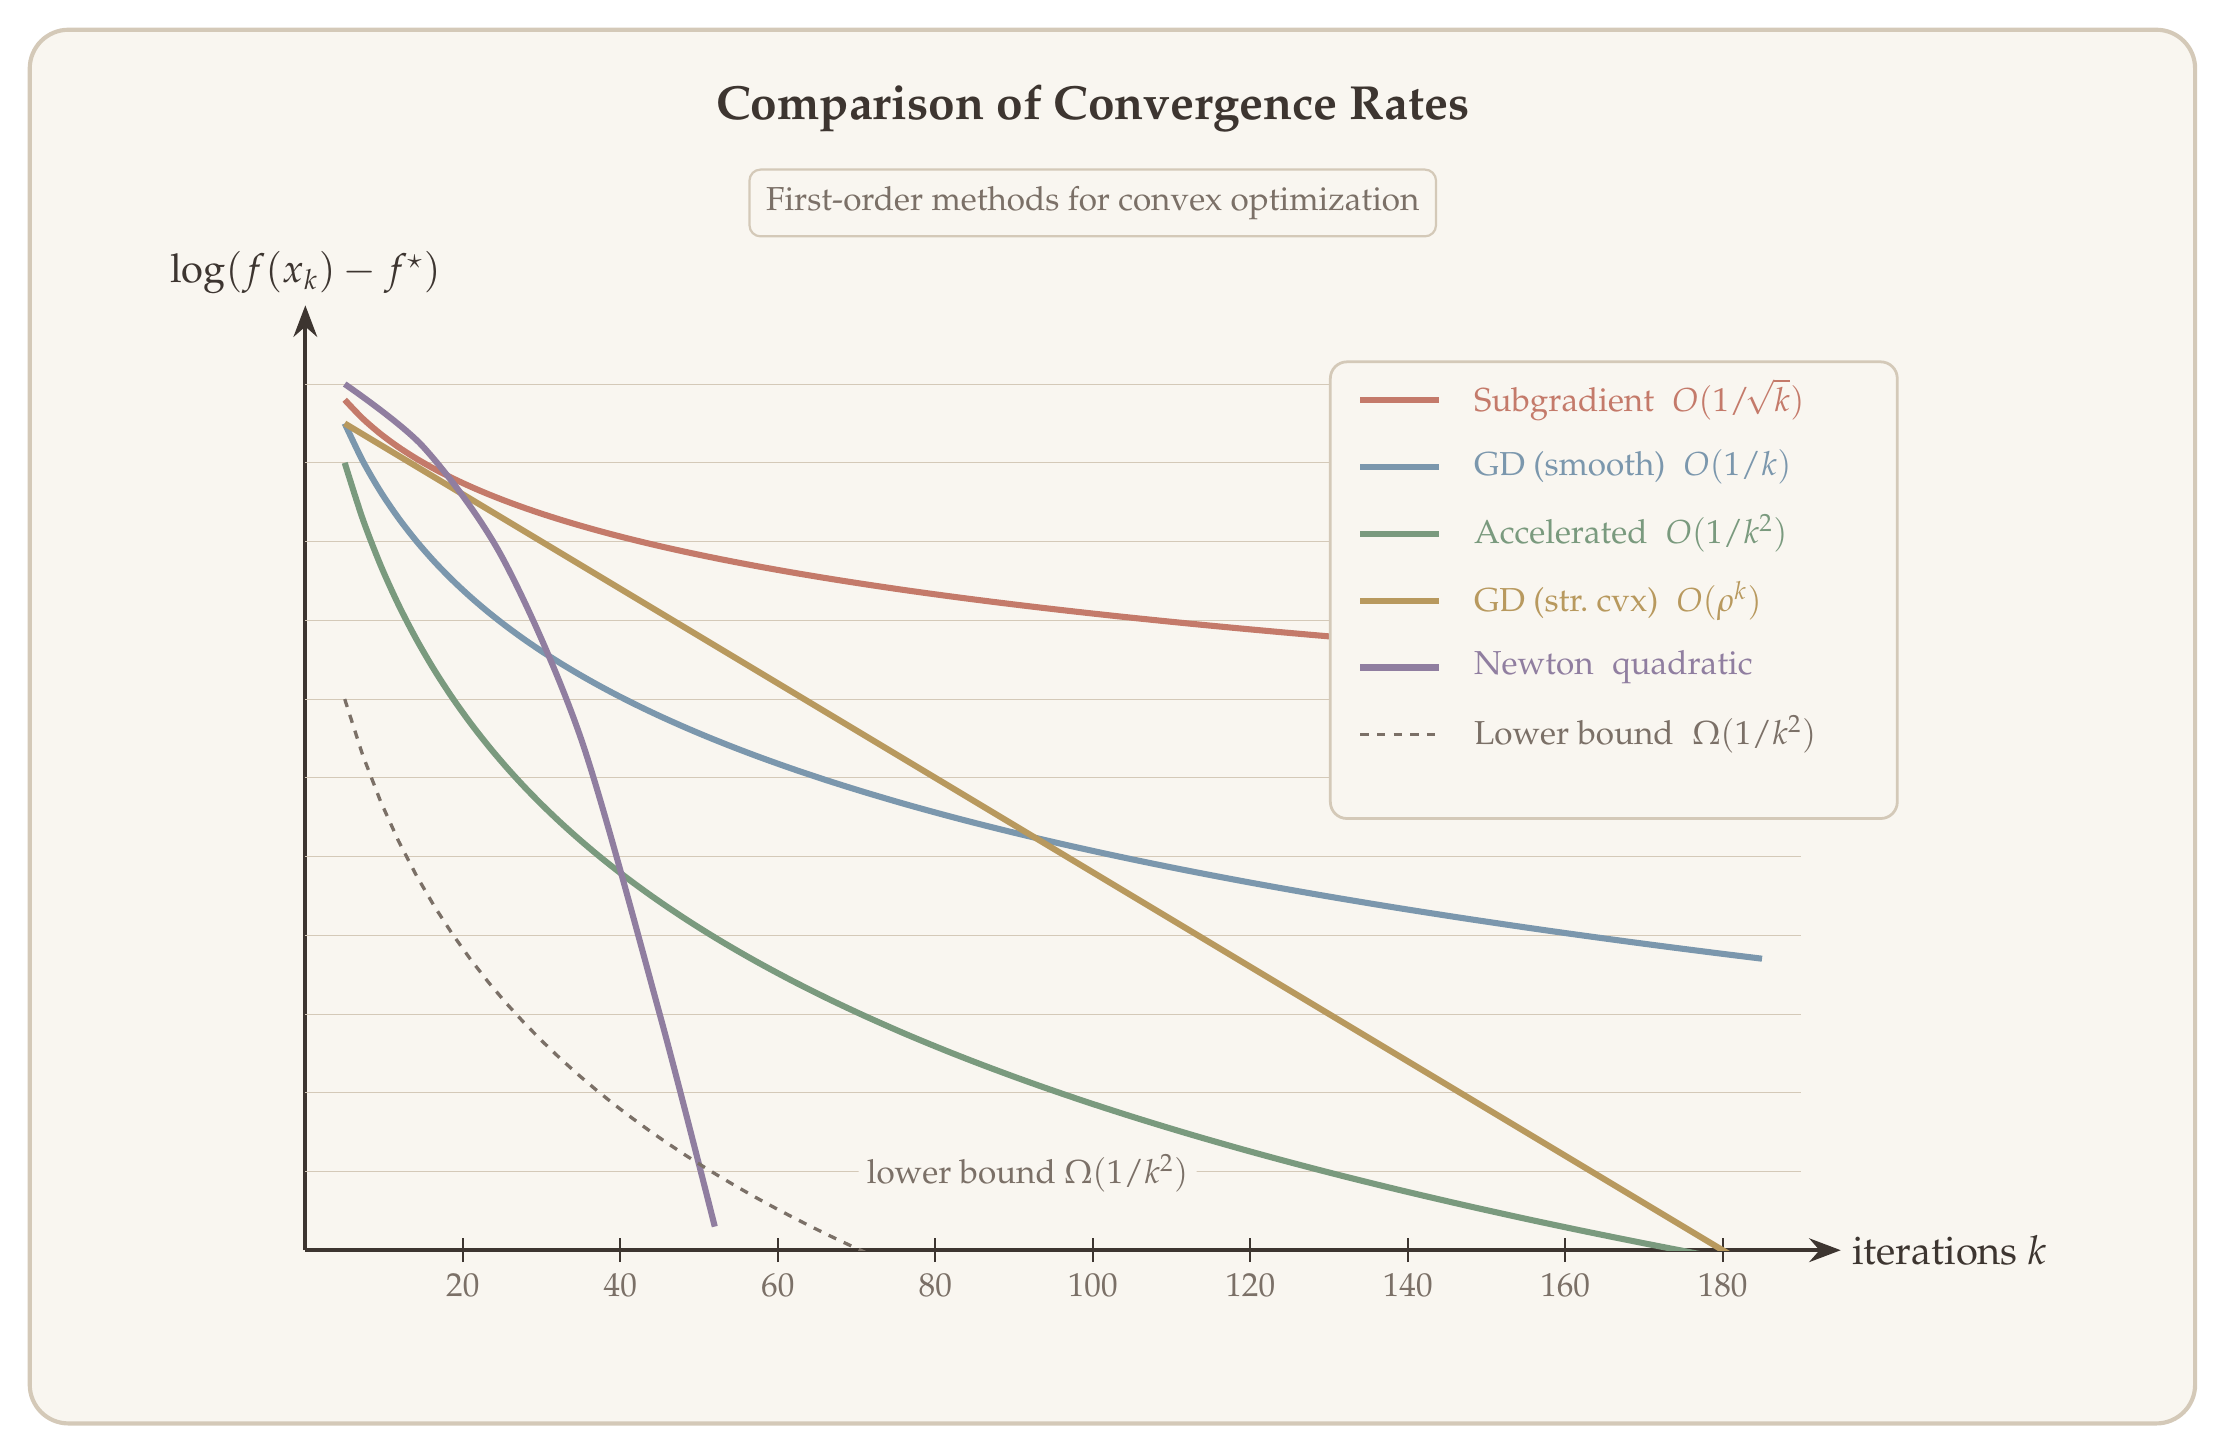
\begin{tikzpicture}[>={Stealth[length=4mm, width=3mm]}, line width=1.5pt]

% Background
\fill[cream, rounded corners=14pt] (-3.5,-2.2) rectangle (24,15.5);
\draw[border, line width=1.5pt, rounded corners=14pt] (-3.5,-2.2) rectangle (24,15.5);

% Title
\node[font=\LARGE\bfseries, text=dkbrown] at (10,14.5) {Comparison of Convergence Rates};

% Subtitle
\node[fill=cream, draw=border, line width=0.8pt, rounded corners=4pt,
      font=\large, text=wmgray, inner sep=6pt]
  at (10,13.3) {First-order methods for convex optimization};

% Axes
\draw[->, dkbrown, line width=1.5pt] (0,0) -- (19.5,0)
  node[right, font=\Large, text=dkbrown] {iterations $k$};
\draw[->, dkbrown, line width=1.5pt] (0,0) -- (0,12)
  node[above, font=\Large, text=dkbrown] {$\log(f(x_k) - f^\star)$};

% Tick marks on x-axis
\foreach \x/\lab in {2/20, 4/40, 6/60, 8/80, 10/100, 12/120, 14/140, 16/160, 18/180} {
  \draw[dkbrown, line width=0.8pt] (\x,-0.15) -- (\x,0.15);
  \node[font=\large, text=wmgray, below] at (\x,-0.15) {\lab};
}

% Grid lines (faint)
\foreach \y in {1,2,...,11} {
  \draw[border, line width=0.3pt] (0,\y) -- (19,\y);
}

% ── Curves ──
% All start at different y-values near x=0.5 for visual separation.
% Plot area: x in [0,19], y in [0,11.5].
% Design: subgradient stays high; GD smooth moderate; accelerated steeper;
% strongly convex linear crossing; Newton near-vertical drop.

\begin{scope}
  \clip (0,0) rectangle (19,11.5);

  % 1. Subgradient: O(1/sqrt(k)) -- very slow, barely drops
  %    At x=0.5: ~11.0;  at x=18: ~10.8 - 0.8*ln(18.5)/ln(2) ~ 10.8 - 3.3 = 7.5
  \draw[terracotta, line width=2.2pt, smooth, samples=80, domain=0.5:18.5]
    plot (\x, {10.8 - 0.8*ln(\x+0.5)/ln(2)});

  % 2. GD smooth convex: O(1/k) -- moderate drop
  %    At x=0.5: ~10.5;  at x=18: ~10.5 - 1.6*ln(18.5)/ln(2) ~ 10.5 - 6.6 = 3.9
  \draw[stblue, line width=2.2pt, smooth, samples=80, domain=0.5:18.5]
    plot (\x, {10.5 - 1.6*ln(\x+0.5)/ln(2)});

  % 3. Accelerated GD: O(1/k^2) -- steeper
  %    At x=0.5: ~10.0;  at x=18: ~10.0 - 2.4*ln(18.5)/ln(2) ~ 10.0 - 9.9 = 0.1
  \draw[sage, line width=2.2pt, smooth, samples=80, domain=0.5:18.5]
    plot (\x, {10.0 - 2.4*ln(\x+0.5)/ln(2)});

  % 4. GD strongly convex: linear rate (straight line on log scale)
  %    Starts high at y~10.8, crosses subgradient/GD, ends near 0
  %    At x=0.5: 10.8 - 0.3 = 10.5;  at x=17: 10.8 - 10.2 = 0.6
  \draw[rwgold, line width=2.2pt, domain=0.5:18.5]
    plot (\x, {10.8 - 0.6*\x});

  % 5. Newton: quadratic convergence -- drops in ~5 iterations
  \draw[lavender, line width=2.2pt, smooth, tension=0.5]
    plot coordinates {(0.5,11.0) (1.5,10.2) (2.5,8.8) (3.5,6.5) (4.5,3.0) (5.2,0.3)};

  % Lower bound (dashed) -- Omega(1/k^2), same rate as accelerated but lower
  %    At x=0.5: ~7.0;  at x=18: ~7.0 - 2.4*4.12 = -2.9 (clipped ~x=12)
  \draw[wmgray, line width=1.2pt, dashed, samples=80, domain=0.5:18.5]
    plot (\x, {7.0 - 2.4*ln(\x+0.5)/ln(2)});

\end{scope}

% Lower bound label -- positioned along the dashed curve, right of Newton
% At x=7: y = 7.0 - 2.4*ln(7.5)/ln(2) = 7.0 - 6.89 = 0.11 (near x-axis)
% Place slightly above at y=0.6 near x=7
\node[font=\large, text=wmgray, fill=cream, inner sep=3pt, rounded corners=2pt,
      anchor=south west]
  at (7,0.6) {lower bound $\Omega(1/k^2)$};

% ── Legend box (top-right inside plot area, drawn with TikZ lines) ──
\begin{scope}
  % Legend background
  \node[anchor=north west, fill=cream, draw=border, line width=1pt,
        rounded corners=6pt, minimum width=7.2cm, minimum height=5.8cm,
        inner sep=0pt] (legbg) at (13,11.3) {};

  % Row coordinates
  \def\legx{13.4}       % left edge of line swatches
  \def\legxe{14.4}      % right edge of line swatches
  \def\legtx{14.7}      % text start
  \def\legy{10.8}       % first row y
  \def\legdy{0.85}      % row spacing

  % Row 1: Subgradient
  \draw[terracotta, line width=2.2pt] (\legx,\legy) -- (\legxe,\legy);
  \node[anchor=west, font=\large, text=terracotta] at (\legtx,\legy)
    {Subgradient\;\;$O(1/\!\sqrt{k})$};

  % Row 2: GD (smooth)
  \pgfmathsetmacro{\rowB}{\legy - \legdy}
  \draw[stblue, line width=2.2pt] (\legx,\rowB) -- (\legxe,\rowB);
  \node[anchor=west, font=\large, text=stblue] at (\legtx,\rowB)
    {GD (smooth)\;\;$O(1/k)$};

  % Row 3: Accelerated
  \pgfmathsetmacro{\rowC}{\legy - 2*\legdy}
  \draw[sage, line width=2.2pt] (\legx,\rowC) -- (\legxe,\rowC);
  \node[anchor=west, font=\large, text=sage] at (\legtx,\rowC)
    {Accelerated\;\;$O(1/k^2)$};

  % Row 4: GD (str. cvx)
  \pgfmathsetmacro{\rowD}{\legy - 3*\legdy}
  \draw[rwgold, line width=2.2pt] (\legx,\rowD) -- (\legxe,\rowD);
  \node[anchor=west, font=\large, text=rwgold] at (\legtx,\rowD)
    {GD (str.\ cvx)\;\;$O(\rho^k)$};

  % Row 5: Newton
  \pgfmathsetmacro{\rowE}{\legy - 4*\legdy}
  \draw[lavender, line width=2.2pt] (\legx,\rowE) -- (\legxe,\rowE);
  \node[anchor=west, font=\large, text=lavender] at (\legtx,\rowE)
    {Newton\;\;quadratic};

  % Row 6: Lower bound
  \pgfmathsetmacro{\rowF}{\legy - 5*\legdy}
  \draw[wmgray, line width=1.2pt, dashed] (\legx,\rowF) -- (\legxe,\rowF);
  \node[anchor=west, font=\large, text=wmgray] at (\legtx,\rowF)
    {Lower bound\;\;$\Omega(1/k^2)$};
\end{scope}

\end{tikzpicture}
\end{document}
